\chapter{Trigonometria}
\section{Trigonometria no Triângulo Retângulo}
%Para realizar o estudo de triângulos retângulos, como na medida da altura de prédios e  árvores ou na largura de rios, podemos utilizar como um modelo um triângulo semelhante ao estudado, mas menor (ou maior, caso o problema envolva uma dimensão muito pequena). Dessa forma, podemos ver que a razão entre os lados dos triângulos é constante, e podemos estudar esta relação.
\begin{figure}[H]
	\centering
    \resizebox{.7\textwidth}{!}{
	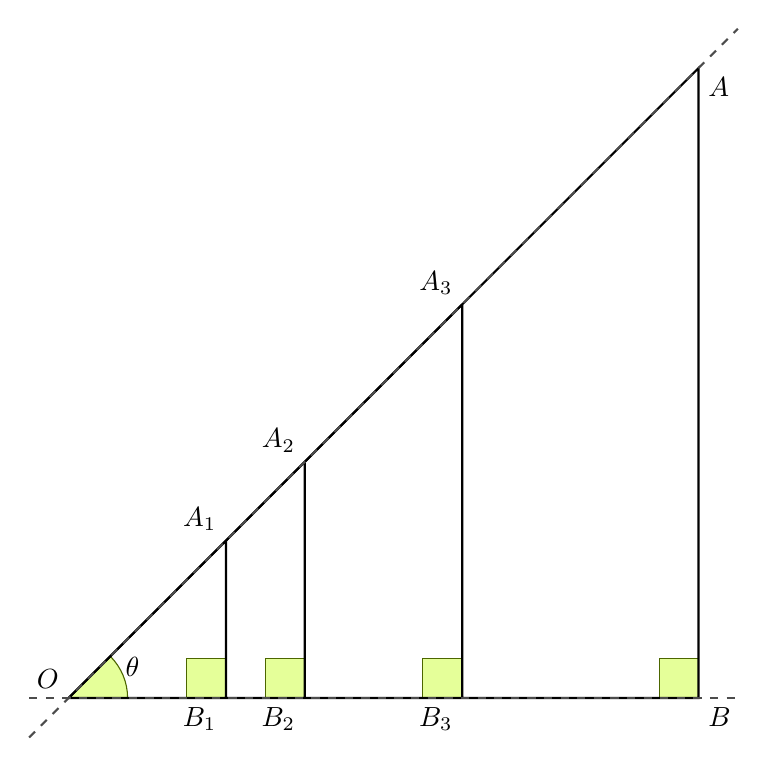
\begin{tikzpicture}
        \filldraw[fill = white!60!lime, draw=black!60!lime] (0,0) -- (0.75,0) arc (0:45:0.75) -- (0,0);
        \filldraw[fill = white!60!lime!, draw=black!60!lime] (4.5,0) rectangle (5,0.5);
        \filldraw[fill = white!60!lime!, draw=black!60!lime] (1.5,0) rectangle (2,0.5);
        \filldraw[fill = white!60!lime!, draw=black!60!lime] (2.5,0) rectangle (3,0.5);
        \filldraw[fill = white!60!lime!, draw=black!60!lime] (7.5,0) rectangle (8,0.5);
        \draw[thick] (0,0) -- (5,0) -- (5,5) -- (3,3) -- (3,0) -- (2,0) -- (2,2) -- (0,0) -- (8,0) -- (8,8) -- (0,0);
        \draw[thick] (0,0) -- (5,5);
      \draw[thick,gray!60!black,dashed] (-0.5,-0.5) -- (8.5,8.5);  \draw[thick,gray!60!black,dashed] (-0.5,0) -- (8.5,0);
      \draw (0,0) node[above left] {$O$};
      \draw (8,0) node[below right] {$B$};
      \draw (8,8) node[below right] {$A$};
      \draw (2,2) node[above left] {$A_1$};
      \draw (3,3) node[above left] {$A_2$};
      \draw (5,5) node[above left] {$A_3$};
      \draw (2,0) node[below left] {$B_1$};
      \draw (3,0) node[below left] {$B_2$};
      \draw (5,0) node[below left] {$B_3$};
      \draw (0.6,0.4) node[right] {$\theta$};
	\end{tikzpicture}}
\end{figure}
Consideremos um ângulo $A\hat{O}B =\theta$, $0\degree<\theta<90\degree$, e tracemos a partir dos pontos $A_1, A_2, A_3 \in \overrightarrow{OA}$ segmentos $\overline{A_1B_1},\overline{A_2B_2}, \overline{A_3B_3}$, perpendiculares a $\overrightarrow{OB}$, como na figura acima. Estão construídos, assim, triângulos retângulos.

\begin{exemplo}
Sejam os triângulos retângulos semelhantes dados na figura abaixo
\begin{figure}[H]
	\centering
    \resizebox{.5\textwidth}{!}{
	\begin{tikzpicture}
		\draw[thick] (0,0) -- (3,0) -- (3,4) -- (0,0) -- (6,0) -- (6,8) -- (0,0) -- (9,0) -- (9,12) -- (0,0);
        \draw (0,0) node[below] {$A$};
        \draw (3,0) node[below] {$B$};
        \draw (3,4) node[above left] {$C$};
        \draw (6,0) node[below] {$D$};
        \draw (9,0) node[below] {$E$};
        \draw (6,8) node[above left] {$F$};
        \draw (9,12) node[above left] {$G$};
        \draw (1.5,0) node[below] {$3$};
        \draw (4.5,0) node[below] {$3$};
        \draw (7.5,0) node[below] {$3$};
        \draw (1.5,2) node[above left] {$5$};
        \draw (4.5,6) node[above left] {$5$};
        \draw (7.5,10) node[above left] {$5$};
        \draw (3,2) node[right] {$4$};
        \draw (6,4) node[right] {$8$};
        \draw (9,6) node[right] {$12$};
	\end{tikzpicture}}
\end{figure}
Assim, \[\sin(C\hat{A}B)=\frac{4}{5}=\frac{8}{10}=\frac{12}{15}\].

\end{exemplo}

A partir da relação de semelhança destes triângulos, temos que
\begin{align*}
\overline{A_1B_1} = k\cdot \overline{OA_1} \\
\overline{A_2B_2} = k\cdot \overline{OA_2} \\
\overline{A_1B_3} = k\cdot \overline{OA_3}
\end{align*}
ou seja,
\[\dfrac{\overline{A_1B_1} }{\overline{OA_1} } =\dfrac{\overline{A_2B_2} }{\overline{OA_2} } =\dfrac{\overline{A_3B_3} }{\overline{OA_3} }=k \]
Assim, esta relação é válida para todos os triângulos semelhantes ao triângulo $\triangle AOB$ e, portanto, a relação depende apenas do ângulo. Logo, definimos ela como função deste ângulo:
\[\dfrac{\overline{A_1B_1} }{\overline{OA_1} } =\dfrac{\overline{A_2B_2} }{\overline{OA_2} } =\dfrac{\overline{A_3B_3} }{\overline{OA_3} }=\sin \theta \]
Tomando outros lados do triângulo, podemos estabelecer razões - e portanto funções - diferentes.
\[\dfrac{\overline{OB_1} }{\overline{OA_1} } =\dfrac{\overline{OB_2} }{\overline{OA_2} } =\dfrac{\overline{OB_3} }{\overline{OA_3} }=\cos \theta \]
\[\dfrac{\overline{A_1B_1} }{\overline{OB_1} } =\dfrac{\overline{A_2B_2} }{\overline{OB_2} } =\dfrac{\overline{A_3B_3} }{\overline{OB_3} }=\tan \theta \]
Podemos definir estas relações facilmente no triângulo abaixo.

% O QUE É OPOSTO E O QUE É O ADJACENTE?
\begin{df}
Seja $\triangle ABC$ retângulo em $A$.
\begin{figure}[H]
	\centering
	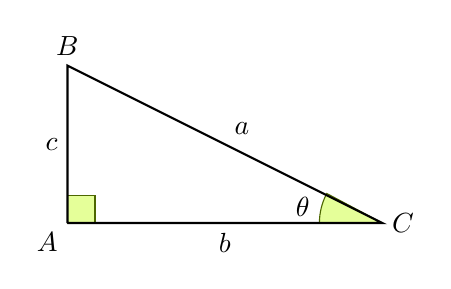
\begin{tikzpicture}
        \filldraw[fill = white!60!lime, draw=black!60!lime] (0,0) -- (0.35,0) -- (0.35,0.35) -- (0,0.35) -- (0,0);
        \filldraw[fill = white!60!lime, draw=black!60!lime] (3.2,0) arc (180:152:0.8) -- (4,0);
		\draw[thick] (0,0) -- (4,0) -- (0,2) -- (0,0);
        \draw (0,1) node[left] {$c$};
        \draw (2,0) node[below] {$b$};
        \draw (2,1) node[above right] {$a$};
        \draw (0,0) node[below left] {$A$};
        \draw (4,0) node[right] {$C$};
        \draw (0,2) node[above] {$B$};
        \draw (3.2,0.2) node[left] {$\theta$};
	\end{tikzpicture}
\end{figure}


A partir deste triângulo, temos que 
\begin{align*}
&\sin \theta = \dfrac{c}{a}=\dfrac{\text{cateto oposto}}{\text{hipotenusa}}\\
&\cos \theta = \dfrac{b}{a}=\dfrac{\text{cateto adjacente}}{\text{hipotenusa}}\\
&\tan \theta = \dfrac{c}{b}=\dfrac{\text{cateto oposto}}{\text{cateto adjacente}}
\end{align*}
\end{df}
Várias relações podem ser formadas a partir destas definições, como consequências da construção do triângulo retângulo. 
\begin{prop}
\[\tan \theta = \dfrac{\sin \theta}{\cos \theta}\]
\begin{proof}
\begin{align*}
\tan \theta &= \dfrac{b}{c} \\
&=\dfrac{b}{a} \cdot \dfrac{a}{c} \\
&= \dfrac{b}{a} : \dfrac{c}{a} \\
&= \dfrac{\sin \theta}{\cos \theta}
\end{align*}
\end{proof}
\end{prop}
\begin{prop}[Relação Fundamental da Trigonometria]
\[\sin^2 \theta + \cos^2 \theta = 1\]
\begin{proof}
\begin{align*}
\sin^2\theta + \cos^2\theta &= \left(\dfrac{b}{a}\right)^2 + \left( \dfrac{c}{a}\right)^2 \\
&= \dfrac{b^2}{a^2}+\dfrac{c^2}{a^2}\\
&= \dfrac{b^2 + c^2}{a^2}
\end{align*}
Sendo $\triangle ABC$ retângulo em $A$, temos que $a^2=b^2+c^2$. Portanto
\begin{align*}
\sin^2\theta + \cos^2\theta &=\dfrac{a^2}{a^2} \\
&= 1
\end{align*}
\end{proof}
\end{prop}
\begin{prop}
Se dois ângulos $\alpha$ e $\beta$ são complementares ($\alpha+\beta=90\degree$), então $\sin \alpha = \cos \beta$ e $\tan\alpha= \frac{1}{\tan\beta}$.
\begin{proof}


\begin{figure}[H]
\centering
	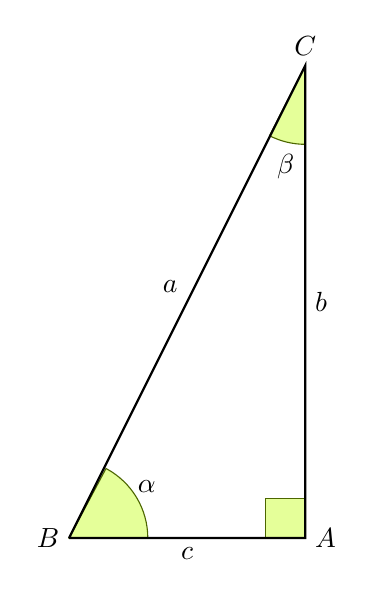
\begin{tikzpicture}
        \filldraw[fill = white!60!lime, draw=black!60!lime] (1,0) arc (0:62:1) -- (0,0) -- (1,0);
		\filldraw[fill = white!60!lime, draw=black!60!lime] (3,5) arc (270:243:1) -- (3,6) -- (3,5);
    \filldraw[fill = white!60!lime, draw=black!60!lime] (3,0) -- (2.5,0) -- (2.5,0.5) -- (3,0.5) -- (3,0);
	\draw[thick] (0,0) -- (3,0) -- (3,6) -- (0,0);
    \draw (0.75,0.65) node[right] {$\alpha$};
    \draw (2.75,5) node[below] {$\beta$};
    \draw (0,0) node[left] {$B$};
    \draw (3,0) node[right] {$A$};
    \draw (3,6) node[above] {$C$};
    \draw (3,3) node[right] {$b$};
    \draw (1.5,3) node[above left] {$a$};
    \draw (1.5,0) node[below] {$c$};
	\end{tikzpicture}
\end{figure}

\[\sin \alpha = \dfrac{b}{a} = \cos \beta\]
\[\tan \alpha = \dfrac{b}{c}=\dfrac{1}{\frac{c}{b}}= \dfrac{1}{\tan \beta}\]
\end{proof}
\end{prop}
Além destas propriedades, podemos gerar várias outras, através da construção de triângulos retângulos. Assim, seguem as relações a seguir.
\begin{prop}
Se $\theta \in (0\degree;45\degree)$, então $\sin (2\theta) = 2\cdot\sin\theta\cdot\cos\theta$. Se $\theta \in (0\degree; 90\degree)$, então $\sin \frac{\theta}{2}=\sqrt{\frac{1-\cos \theta}{2}}$.
\begin{proof}
\begin{figure}[H]   %PARA QUEM QUISER PLOTAR ESTA IMAGEM LINDA
\centering
\includegraphics[width=0.8\textwidth]{basic/images/trigo4}
\end{figure}
Esta figura é formada por dois triângulos, $\triangle OAB$ e $\triangle OAC$ congruentes, retângulos em $A$, tais que $\overline{OB}=\overline{OC}=1$ e $A\hat{O}B = A\hat{O}C = \theta$. Nestas condições, temos $\overline{AB}=\overline{AC}=\sin \theta$ e $\overline{OA}=\cos \theta$. Traçando $\overline{BD}$ perpendicular a $\overline{OC}$ temos ainda $\overline{BD}=\sin(2\theta)$. O dobro da área de $\triangle OBC$ é igual a $\overline{BC}\cdot\overline{OA}$ e também igual a $\overline{OC}\cdot\overline{BD}$. Portanto,
\begin{align*}
\overline{BC}\cdot\overline{OA} &= \overline{OC}\cdot\overline{BD}\\
(\overline{AB} + \overline{AC})\cdot \cos \theta &= 1 \cdot \sin(2\theta) \\
(\sin\theta+\sin\theta)\cos\theta &= \sin(2\theta) \\
2\sin\theta\cos\theta &= \sin(2\theta)
\end{align*}
Observemos que $\overline{OD}+\overline{DC}=1$, ou $1\cdot\cos(2\theta)+\overline{BC}\cdot\cos\beta=1$. Como $\overline{BC}=2\cdot \sin \theta $ e $\cos \beta = \sin \theta$ ($\theta$ e $\beta$ são complementares), temos
\[cos(2\theta)+2\sin(\theta)\cdot\sin(\theta)=1\]
ou ainda, \[\sin \theta = \sqrt{\dfrac{1-cos(2\theta)}{2}}\]
Substituindo $2\theta$ por $\theta$ e consequentemente $\theta$ por $\frac{\theta}{2}$, obtemos a relação procurada.
\end{proof}
\end{prop}